\section{分布式账本的扩容问题}

本节从数字货币的双花问题出发,分析区块链扩容的难点的根源是什么。
然后对比所有权交割与债权清算在这个问题上的差异。
从中总结为什么闪电网络能够摆脱三元不可能原理的束缚,从根本上提高支付的吞吐量。
从宏观上理解闪电网络的原理,有助于读者理解微观的技术细节。

\subsection{数字货币的确权问题与双花问题}

从货币的历史上看,货币的去实物化是长期存在的发展趋势。从粮食、到黄金、再到纸钞,货币本身的内在价值逐步减小。
货币的内涵不依赖于其自身的价值,而依赖于它代表的价值,或者说依赖于人们认为它代表的价值。
所以货币的材质、形状、颜色、图案这些因素不是货币的本质,随着货币的发展这些因素都在不断的变化。
货币的最终极形态是数字货币,完全去实物化,彻底摆脱外在的实物载体的限制。
数字货币的优点很多,包括便于储藏、转移,易分割,同时在防抢劫、防盗窃等方面有更好的安全性。

虽然数字货币有诸多优点,但是长期以来人们一直使用实物货币,数字货币很晚才出现。
很重要的原因是由于数字货币有两个特有的问题需要解决:
\begin{itemize}
  \item \textbf{确权问题}:谁是某一笔货币的拥有者?
  \item \textbf{双花问题}:某一笔货币是不是已经被花出去了?
\end{itemize}

由于实物货币具有不可复制性,这两个问题很容易解决。
但是由于数字货币的复制成本几乎为零,解决方案就不是那么简单了。
其中的确权问题相对比较容易,可以通过数字签名可以确定所有权。下面重点讨论双花问题。

\subsection{所有权交割的模式}
比特币是一种端到端的电子货币系统,类似于现金支付的过程,它使用的是所有权交割的模式完成支付。
如图~\ref{fig:gossip} 是一个日常的支付场景,Alice 向 Bob 支付 10 美元。
假如这10美元是实物钞票,那么Bob 只需要验证钞票的真伪即可,不需要关心双花的问题。
但对于 10 美元的数字货币,Bob 没有简单的办法确认这 10 美元是否已经被 Alice 花费给了其他人。
这个问题的困难在于,Alice 可以把数字货币的所有权转给任何人,所以 Bob 需要访问所有可能的接受者,才能确认 Alice 之前没有花费这 10 美元。

\begin{figure}[h!]
    \centering
    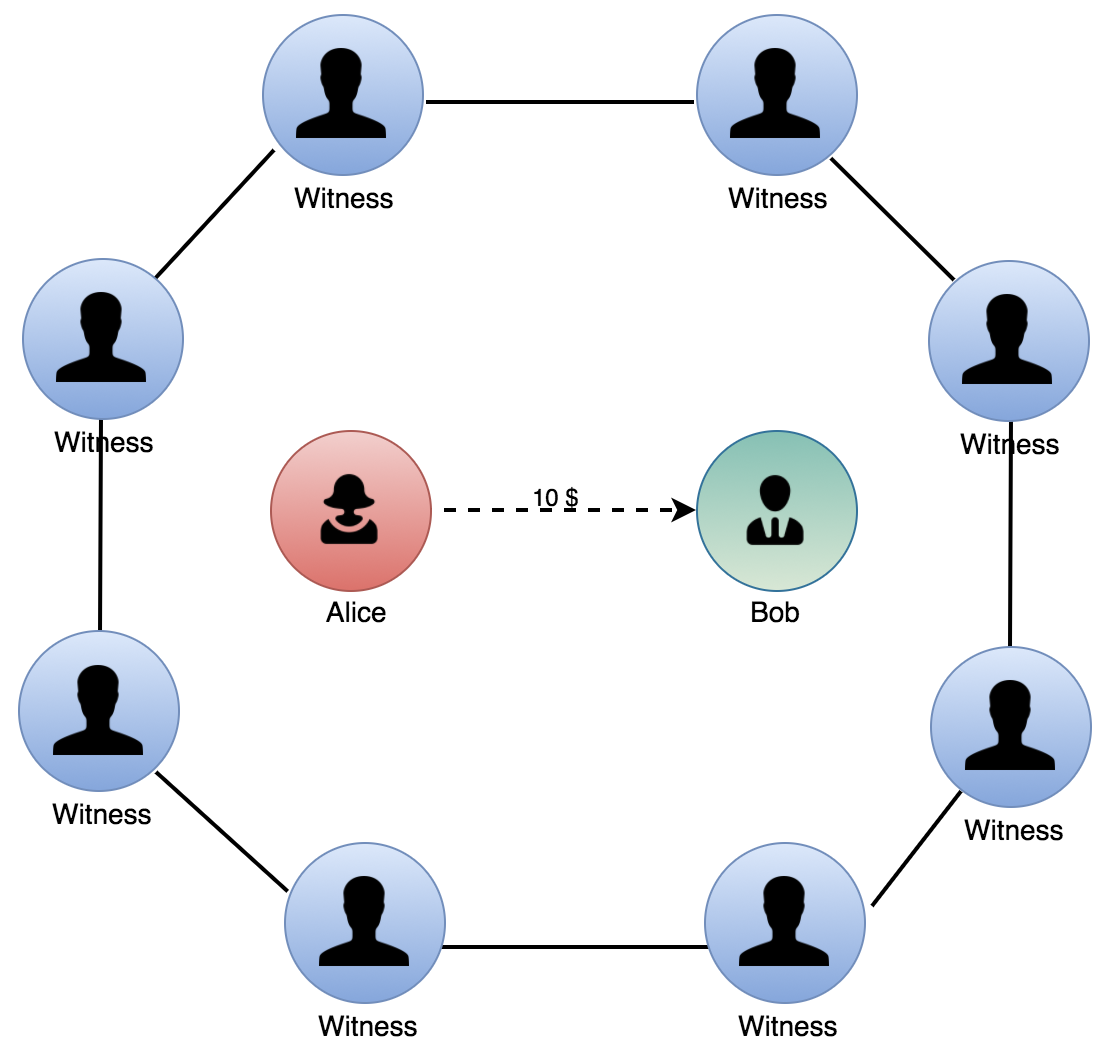
\includegraphics[width=8cm, keepaspectratio]{../images/Gossip.png}
    \caption{}
    \label{fig:gossip}
\end{figure}
\newpage
显然穷举并且访问所有人是不可行的。对于这个问题,中本聪在比特币的创世论文中提到:

\begin{quote}
    \textbf{\textit{We need a way for the payee to know that the previous owners did not sign any earlier transactions. 
            For our purposes, the earliest transaction is the one that counts, so we don't care about later attempts to double-spend. 
            The only way to confirm the absence of a transaction is to be aware of all transactions.}}
\end{quote}

中本聪的解决办法是构建一个分布式账本,包含所有历史交易记录。
Bob 根据这个账本直接验证 Alice 是否已经花费了这 10 美元,免去了遍历所有的参与者的麻烦。
但是分布式账本需要众多的节点共同维护,这些节点独立管理一份全量副本。
为了保证各个节点之间的一致性,同时规避拜占庭故障问题,每一笔交易都要交给所有矿工见证。
见证的过程中再附加上工作量证明,令攻击者必须要付出更多工作量才能篡改交易的历史记录。
所以每一笔交易的处理成本与节点的个数是正相关的,代价非常高昂。

我们来定性的分析一下。假设参与共识的节点为 $N$,
每笔交易消耗的成本(存储、通信、计算)复杂度均为 O(N),分布式账本每秒消耗的成本。那么有公式:

\begin{gather}\label{equ:cost}
\text{每秒消耗的资源}_\text{存储} = \text{吞吐量(TPS)} \times O(N) \\
\text{每秒消耗的资源}_\text{通信} = \text{吞吐量(TPS)} \times O(N) \\
\text{每秒消耗的资源}_\text{计算} = \text{吞吐量(TPS)} \times O(N) 
\end{gather}

从这个公式可以看到,降低系统成本、提高吞吐量、加强去中心化程度(提高共识节点个数$N$),这三个目标是不可能同时完成的。
这是有分布式账本本身的特点决定的,无论怎样设计一个区块链系统,都不可能超出三元不可能性原理的限制。

%比特币创造性的解决了数字货币的双花问题,经过10年的稳定运行,已经证明了其安全性。
%但是这个解决方案存在天生的运行效率的瓶颈。比特币的平均吞吐量大约是 3~4 TPS,远远无法满足现代支付系统的需求。
%

\subsection{债权清算的支付模式}
回顾上面的分析,我们可以发现,在所有权的交割的模式下,数字货币的支付系统必然会受到三元不可能原理的制约。
那么我们换一个思路,看一下债权清算的情况。银行转账就是通过债权清算的方式完成的。其工作原理如图\ref{fig:clearing}:

\begin{figure}[h!]
    \centering
    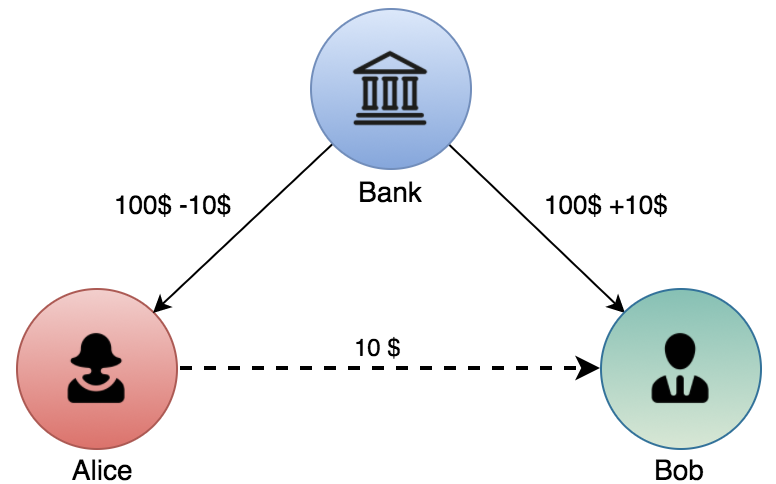
\includegraphics[width=8cm, keepaspectratio]{../images/clearing.png}
    \caption{通过债务清算完成支付}
    \label{fig:clearing}
\end{figure}

Alice 和 Bob 分别在银行里存入 100 美元,或者说银行分别欠 Alice 和 Bob 100 美元。
当 Alice 需要向 Bob 支付 10 美元的时候,银行对 Alice 的债务余额减10美元,对 Bob 的债务余额加10美元。
支付过程中 不需要 Alice 和 Bob 之间交割任何实物货币,只需要银行居间调整债务余额就可以了。

因为相对于所有权交割的支付方式,债务清算可以更加高效的解决双花问题。
如果 Bob 要确认 Alice 没有双花,只需要让银行与 Alice 共同确认当前最新的余额是多少就可以了。
不需要其它任何第三方的参与。相对于比特币的分布式账本来讲,一笔交易的处理成本从 $O(N)$ 降到了 $O(1)$。
从根源上摆脱了三元不可能原理的限制,可以非常有效的提高支付系统的性能。

债务清算的支付方式已经在传统的银行机构大规模普及了,而且获得了很大的成功。
Visa、支付宝等支付系统背后都有银行、清算中心的支撑。
但是因为客户的资产必须长期由银行托管,保持债务关系,
银行必须有强大的信用背书和风控制度,防范各种金融风险,保证银行有充足的偿付能力,以免银行被挤兑。
为此现代金融系统建立了一整套法律和监管体系,防范这些风险的累积和爆发。
然而随着金融体系越来越庞大、越来越复杂,金融监管的成本也越来越高,这些成本最终转化交易的摩擦由消费者买单。

\subsection{闪电网络的思路}
我们对比一下比特币与现代银行系统,二者都是数字货币的支付系统。
如果从性能和去信任性这两个维度对比银行系统和区块链系统,我们看到二者恰好是互补的。
比特币是基于所有权交割的支付系统,采用分布式账本解决双花问题,所以效率低下,但是它的优点是去信任的,不需要金融中介的参与;
反之,银行系统是基于债权清算的支付系统,可以支持高并发、大吞吐量的性能,但是依赖于金融中介的信任,要承担监管和合规的成本。二者像是两个极端,互不相容。

\begin{figure}[h!]
    \centering
    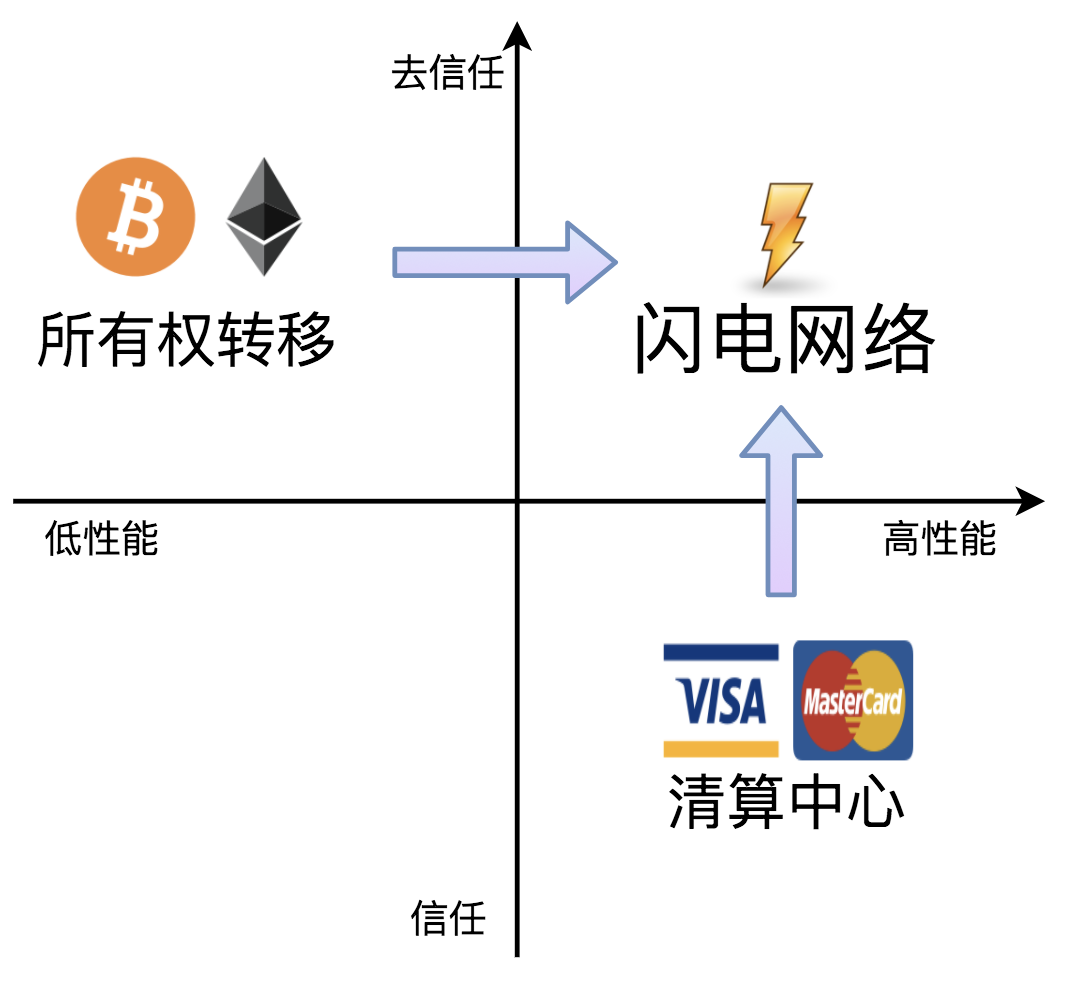
\includegraphics[width=8cm, keepaspectratio]{../images/comparision.png}
    \caption{分布式账本 vs. 银行系统}
    \label{fig:comparition}
\end{figure}

闪电网络巧妙的整合了二者的优点,一方面利用比特币的智能合约维护债务关系,规避了对于金融机构的依赖;
另一方面采用债务清算的方式完成支付,提高了系统的吞吐量。这种新的支付方式我们称之为:基于支付通道的、去信任的、实时清算协议。
